% Options for packages loaded elsewhere
\PassOptionsToPackage{unicode}{hyperref}
\PassOptionsToPackage{hyphens}{url}
\documentclass[
  11pt,
]{article}
\usepackage{xcolor}
\usepackage[margin=1in]{geometry}
\usepackage{amsmath,amssymb}
\setcounter{secnumdepth}{-\maxdimen} % remove section numbering
\usepackage{iftex}
\ifPDFTeX
  \usepackage[T1]{fontenc}
  \usepackage[utf8]{inputenc}
  \usepackage{textcomp} % provide euro and other symbols
\else % if luatex or xetex
  \usepackage{unicode-math} % this also loads fontspec
  \defaultfontfeatures{Scale=MatchLowercase}
  \defaultfontfeatures[\rmfamily]{Ligatures=TeX,Scale=1}
\fi
\usepackage{lmodern}
\ifPDFTeX\else
  % xetex/luatex font selection
\fi
% Use upquote if available, for straight quotes in verbatim environments
\IfFileExists{upquote.sty}{\usepackage{upquote}}{}
\IfFileExists{microtype.sty}{% use microtype if available
  \usepackage[]{microtype}
  \UseMicrotypeSet[protrusion]{basicmath} % disable protrusion for tt fonts
}{}
\makeatletter
\@ifundefined{KOMAClassName}{% if non-KOMA class
  \IfFileExists{parskip.sty}{%
    \usepackage{parskip}
  }{% else
    \setlength{\parindent}{0pt}
    \setlength{\parskip}{6pt plus 2pt minus 1pt}}
}{% if KOMA class
  \KOMAoptions{parskip=half}}
\makeatother
\usepackage{color}
\usepackage{fancyvrb}
\newcommand{\VerbBar}{|}
\newcommand{\VERB}{\Verb[commandchars=\\\{\}]}
\DefineVerbatimEnvironment{Highlighting}{Verbatim}{commandchars=\\\{\}}
% Add ',fontsize=\small' for more characters per line
\newenvironment{Shaded}{}{}
\newcommand{\AlertTok}[1]{\textcolor[rgb]{1.00,0.00,0.00}{\textbf{#1}}}
\newcommand{\AnnotationTok}[1]{\textcolor[rgb]{0.38,0.63,0.69}{\textbf{\textit{#1}}}}
\newcommand{\AttributeTok}[1]{\textcolor[rgb]{0.49,0.56,0.16}{#1}}
\newcommand{\BaseNTok}[1]{\textcolor[rgb]{0.25,0.63,0.44}{#1}}
\newcommand{\BuiltInTok}[1]{\textcolor[rgb]{0.00,0.50,0.00}{#1}}
\newcommand{\CharTok}[1]{\textcolor[rgb]{0.25,0.44,0.63}{#1}}
\newcommand{\CommentTok}[1]{\textcolor[rgb]{0.38,0.63,0.69}{\textit{#1}}}
\newcommand{\CommentVarTok}[1]{\textcolor[rgb]{0.38,0.63,0.69}{\textbf{\textit{#1}}}}
\newcommand{\ConstantTok}[1]{\textcolor[rgb]{0.53,0.00,0.00}{#1}}
\newcommand{\ControlFlowTok}[1]{\textcolor[rgb]{0.00,0.44,0.13}{\textbf{#1}}}
\newcommand{\DataTypeTok}[1]{\textcolor[rgb]{0.56,0.13,0.00}{#1}}
\newcommand{\DecValTok}[1]{\textcolor[rgb]{0.25,0.63,0.44}{#1}}
\newcommand{\DocumentationTok}[1]{\textcolor[rgb]{0.73,0.13,0.13}{\textit{#1}}}
\newcommand{\ErrorTok}[1]{\textcolor[rgb]{1.00,0.00,0.00}{\textbf{#1}}}
\newcommand{\ExtensionTok}[1]{#1}
\newcommand{\FloatTok}[1]{\textcolor[rgb]{0.25,0.63,0.44}{#1}}
\newcommand{\FunctionTok}[1]{\textcolor[rgb]{0.02,0.16,0.49}{#1}}
\newcommand{\ImportTok}[1]{\textcolor[rgb]{0.00,0.50,0.00}{\textbf{#1}}}
\newcommand{\InformationTok}[1]{\textcolor[rgb]{0.38,0.63,0.69}{\textbf{\textit{#1}}}}
\newcommand{\KeywordTok}[1]{\textcolor[rgb]{0.00,0.44,0.13}{\textbf{#1}}}
\newcommand{\NormalTok}[1]{#1}
\newcommand{\OperatorTok}[1]{\textcolor[rgb]{0.40,0.40,0.40}{#1}}
\newcommand{\OtherTok}[1]{\textcolor[rgb]{0.00,0.44,0.13}{#1}}
\newcommand{\PreprocessorTok}[1]{\textcolor[rgb]{0.74,0.48,0.00}{#1}}
\newcommand{\RegionMarkerTok}[1]{#1}
\newcommand{\SpecialCharTok}[1]{\textcolor[rgb]{0.25,0.44,0.63}{#1}}
\newcommand{\SpecialStringTok}[1]{\textcolor[rgb]{0.73,0.40,0.53}{#1}}
\newcommand{\StringTok}[1]{\textcolor[rgb]{0.25,0.44,0.63}{#1}}
\newcommand{\VariableTok}[1]{\textcolor[rgb]{0.10,0.09,0.49}{#1}}
\newcommand{\VerbatimStringTok}[1]{\textcolor[rgb]{0.25,0.44,0.63}{#1}}
\newcommand{\WarningTok}[1]{\textcolor[rgb]{0.38,0.63,0.69}{\textbf{\textit{#1}}}}
\usepackage{longtable,booktabs,array}
\usepackage{caption}
\captionsetup[table]{skip=6pt}
\newcounter{none} % for unnumbered tables
\usepackage{calc} % for calculating minipage widths
% Correct order of tables after \paragraph or \subparagraph
\usepackage{etoolbox}
\makeatletter
\patchcmd\longtable{\par}{\if@noskipsec\mbox{}\fi\par}{}{}
\makeatother
% Allow footnotes in longtable head/foot
\IfFileExists{footnotehyper.sty}{\usepackage{footnotehyper}}{\usepackage{footnote}}
\makesavenoteenv{longtable}
\usepackage{graphicx}
\makeatletter
\newsavebox\pandoc@box
\newcommand*\pandocbounded[1]{% scales image to fit in text height/width
  \sbox\pandoc@box{#1}%
  \Gscale@div\@tempa{\textheight}{\dimexpr\ht\pandoc@box+\dp\pandoc@box\relax}%
  \Gscale@div\@tempb{\linewidth}{\wd\pandoc@box}%
  \ifdim\@tempb\p@<\@tempa\p@\let\@tempa\@tempb\fi% select the smaller of both
  \ifdim\@tempa\p@<\p@\scalebox{\@tempa}{\usebox\pandoc@box}%
  \else\usebox{\pandoc@box}%
  \fi%
}
% Set default figure placement to htbp
\def\fps@figure{htbp}
\makeatother
\setlength{\emergencystretch}{3em} % prevent overfull lines
\providecommand{\tightlist}{%
  \setlength{\itemsep}{0pt}\setlength{\parskip}{0pt}}
\usepackage{bookmark}
\IfFileExists{xurl.sty}{\usepackage{xurl}}{} % add URL line breaks if available
\urlstyle{same}
% fallback for those not using the hyperref driver hyperxmp:
\makeatletter
\@ifundefined{xmpquote}{\newcommand{\xmpquote}[1]{#1}}{}
\makeatother
\hypersetup{
  hidelinks,
  pdfcreator={LaTeX via pandoc}}

\author{}
\date{}

\begin{document}

\section{\texorpdfstring{Learning Stop/Continue Strategies in
\emph{Can\textquotesingle t
Stop}}{Learning Stop/Continue Strategies in Can\textquotesingle t Stop}}\label{learning-stopcontinue-strategies-in-cant-stop}

\textbf{CS 441 Final Project --- Fall 2026}\\
\textbf{Group members:} \emph{{[}add names and net IDs{]}}\\
\textbf{Code:} {[}repository link to be added{]}\\
\textbf{Data and experiment artifacts:} {[}repository link to be added;
see \texttt{cant\_stop\_baselines/runs/}{]}\\
\textbf{Video:} \emph{{[}add 5--6 minute video link{]}}

\subsection{Abstract}\label{abstract}

We study whether machine learning can improve the strategic
Stop/Continue decision in the two-player board game
\emph{Can\textquotesingle t Stop}. The application observes a game state
after a successful roll and chooses either to bank the temporary
progress or risk another roll. We compare a rule-based baseline, a
supervised linear model, Double DQN, and PPO. Dice-pair selection is
held fixed to the Glenn--Aloi constant-weight policy for the main
comparison, so the experiment isolates the Stop/Continue policy.

The strongest retained model is a PPO policy trained from scratch with
domain features and a 60\% Monte Carlo / 40\% smart Rule-of-28 opponent
mixture. On a fresh common evaluation set of 3,000 games per matchup, it
won 64.6\% against Rule28-smart and 55.4\% against the approximate MC
agent. It significantly outperformed the retained DDQN reference by 3.2
percentage points and 2.7 points, respectively, under paired bootstrap
intervals. Two additional seeds support the PPO result: PPO averaged
64.25\% against Rule28-smart and 55.35\% against MC, compared with
59.50\% and 50.40\% for DDQN. However, PPO and the multi-policy Ridge
model were close in direct head-to-head games, so we do not claim
universal superiority. Learned dice pairing and several fine-tuning and
supervised-DNN variants were negative results.

\subsection{1. Problem Description and
Motivation}\label{1-problem-description-and-motivation}

\subsubsection{1.1 Application}\label{11-application}

The proof-of-concept application is an automated
\emph{Can\textquotesingle t Stop} player. Given the board position,
temporary runners, banked progress, the opponent\textquotesingle s
progress, and the result of the current dice pairing, the player decides
whether to:

\begin{itemize}
\tightlist
\item
  \textbf{Continue:} roll again and potentially gain more progress or
  bust; or
\item
  \textbf{Stop:} bank the current temporary progress and pass the turn.
\end{itemize}

The game is a useful decision-making problem because every decision
trades off short-term risk against progress toward claiming three
columns. A simple heuristic can be reasonable, but the value of
continuing depends on the whole board, opponent threats, completed
columns, and the probability of busting.

\subsubsection{1.2 Intended user and use
case}\label{12-intended-user-and-use-case}

The intended user is a person playing or studying
\emph{Can\textquotesingle t Stop}. The application can act as an
opponent, provide a recommendation during a human game, or serve as an
educational tool that explains why a state is risky. The practical
benefit is a reproducible strategy assistant rather than a claim that
the game has one universally optimal move.

\subsubsection{1.3 ML formulation}\label{13-ml-formulation}

This is a two-action sequential decision problem. At each eligible
decision state, the input is a fixed-length vector describing the
current player\textquotesingle s state. The output is a policy over
\texttt{\{Continue,\ Stop\}}. The principal reward is terminal:
\texttt{+1} for a win, \texttt{-1} for a loss, and \texttt{0} otherwise.
The main PPO and DDQN experiments use fixed GA dice pairing, while the
learned-pairing experiments additionally predict a legal pairing action.

The game engine is independent of the policies. It enforces the standard
board heights \texttt{(3,5,7,9,11,13,11,9,7,5,3)}, at most three active
columns, temporary progress loss on a bust, and victory after three
claimed columns. The implementation was checked by a regression suite
and seeded reproducibility tests.

\subsection{2. ML Approach}\label{2-ml-approach}

\subsubsection{2.1 Baselines}\label{21-baselines}

We used several increasingly strong baselines:

\begin{enumerate}
\def\labelenumi{\arabic{enumi}.}
\tightlist
\item
  \textbf{Rule28-smart:} a transparent heuristic based on Rule of 28 and
  Glenn--Aloi constant move weights. It stops at a score threshold or
  when a temporary runner reaches a column top.
\item
  \textbf{Approximate MC:} fixed GA pairing plus one-turn Monte Carlo
  rollouts, with Rule28-smart used after simulated actions. It is an
  approximate remainder-of-turn policy, not full-game MCTS.
\item
  \textbf{Ridge-domain:} a supervised Ridge regressor predicting the
  approximate margin \texttt{Q(Continue)\ -\ Q(Stop)} from domain
  features. It continues when the predicted margin is positive.
\item
  \textbf{MC-counterfactual DDQN:} the retained RL reference, trained
  with Double DQN, five-step returns, domain features, and
  counterfactual MC supervision.
\end{enumerate}

The final report focuses on PPO, DDQN, and Ridge because Random Forest
and the single-source and multi-policy DNNs were clearly weaker in
complete-game evaluation.

\subsubsection{2.2 PPO model}\label{22-ppo-model}

The promoted PPO policy uses a 68-value domain observation and a 128x128
MLP. It was trained for 100,000 episodes with terminal-only reward,
512-step rollouts, four PPO epochs, minibatches of 256, learning rate
\texttt{1e-4}, and fixed GA pairing. The training opponent mixture was
60\% MC and 40\% Rule28-smart. Training MC used 16 rollouts and a
future-roll limit of 20; held-out evaluation used MC-64. The promoted
checkpoint is the best validation checkpoint from seed 451, episode
95,021:

\texttt{cant\_stop\_baselines/runs/ppo\_mc\_focused\_seed451/top\_1.pt}

Checkpoint selection maximized the minimum validation win rate across
the two primary opponents. We retained the checkpoint rather than the
final training weights because validation performance oscillated
substantially during PPO training.

\subsubsection{2.3 DDQN model}\label{23-ddqn-model}

The DDQN reference uses a 128x128 network, 68 domain features, five-step
returns, fixed GA pairing, terminal game rewards, and an opponent
mixture of Rule28-smart, MC, pure GA Rule 28, classic Rule 28, and
random agents. The retained checkpoint is:

\texttt{cant\_stop\_baselines/runs/ddqn\_mc\_counterfactual\_seed447/best.pt}

This model is the main RL baseline because it was selected before the
final PPO comparison and remained more reliable than attempted self-play
and fine-tuning variants.

\subsubsection{2.4 Supervised Ridge
model}\label{24-supervised-ridge-model}

We collected 10,000 decision states from simulator-generated games. For
each state, the pipeline forced Stop and Continue using shared future
random seeds and estimated each action\textquotesingle s full-game win
probability with paired rollouts. The target was the resulting action
margin. A grouped 70/15/15 split by source game prevented states from
the same game appearing in multiple splits. The multi-policy Ridge model
was trained on states drawn from five policies (Rule28-smart, MC, Ridge,
PPO, and DDQN), using the same counterfactual label procedure. This
distribution improved Ridge robustness over the original single-policy
dataset.

\subsection{3. Data Collection and
Curation}\label{3-data-collection-and-curation}

All data were generated by our own simulator rather than taken from
Kaggle, benchmark datasets, or a pre-curated ML dataset. Each generated
game records the seed, seat assignment, winner, turns, rolls, busts, and
stops. Decision states are stored with fixed-length features and
metadata identifying the source game and policy.

The state representation contains 58 raw values. The domain
representation contains 68 values, including active/top marker counts,
immediate completion and win indicators, board-progress lead,
risk-adjusted turn progress, normalized Rule-of-28 score, and opponent
threat. The strategic ablation adds per-column temporary progress and
completion-threat features.

For supervised labels, the same state and future random seeds were used
for the forced Stop and forced Continue branches. This reduces label
noise caused by unrelated dice variation. Labels remain approximate
because the rollout policy after the forced action is Rule28-smart; they
are not optimal-game ground truth. Source games, rather than individual
states, were split before training. Evaluation games were generated with
fresh seeds that were not used for collection, training, or checkpoint
selection.

For every formal model comparison, seats were alternated. The two games
in a seat-swapped pair share a dice seed, so paired bootstrap is more
appropriate than treating all game outcomes as independent. We report
5,000 paired bootstrap samples and interpret intervals as descriptive
paired inference.

\subsection{4. Experimental Design}\label{4-experimental-design}

\subsubsection{4.1 Primary evaluation}\label{41-primary-evaluation}

The final common evaluation used seed \texttt{1000454}, 3,000 games per
matchup, alternating seats, MC-64, and 5,000 paired-bootstrap samples.
All models faced the same fresh dice seeds and the same two primary
opponents.

\subsubsection{4.2 Primary results}\label{42-primary-results}

{\def\LTcaptype{none} % do not increment counter
\begin{longtable}[]{@{}lrrr@{}}
\toprule\noalign{}
Model & Rule28-smart & MC & Minimum \\
\midrule\noalign{}
\endhead
\bottomrule\noalign{}
\endlastfoot
\textbf{PPO-451 + GA} & \textbf{64.6\%} & \textbf{55.4\%} &
\textbf{55.4\%} \\
DDQN reference & 61.4\% & 52.7\% & 52.7\% \\
Ridge-domain & 60.1\% & 51.1\% & 51.1\% \\
\end{longtable}
}

\pandocbounded{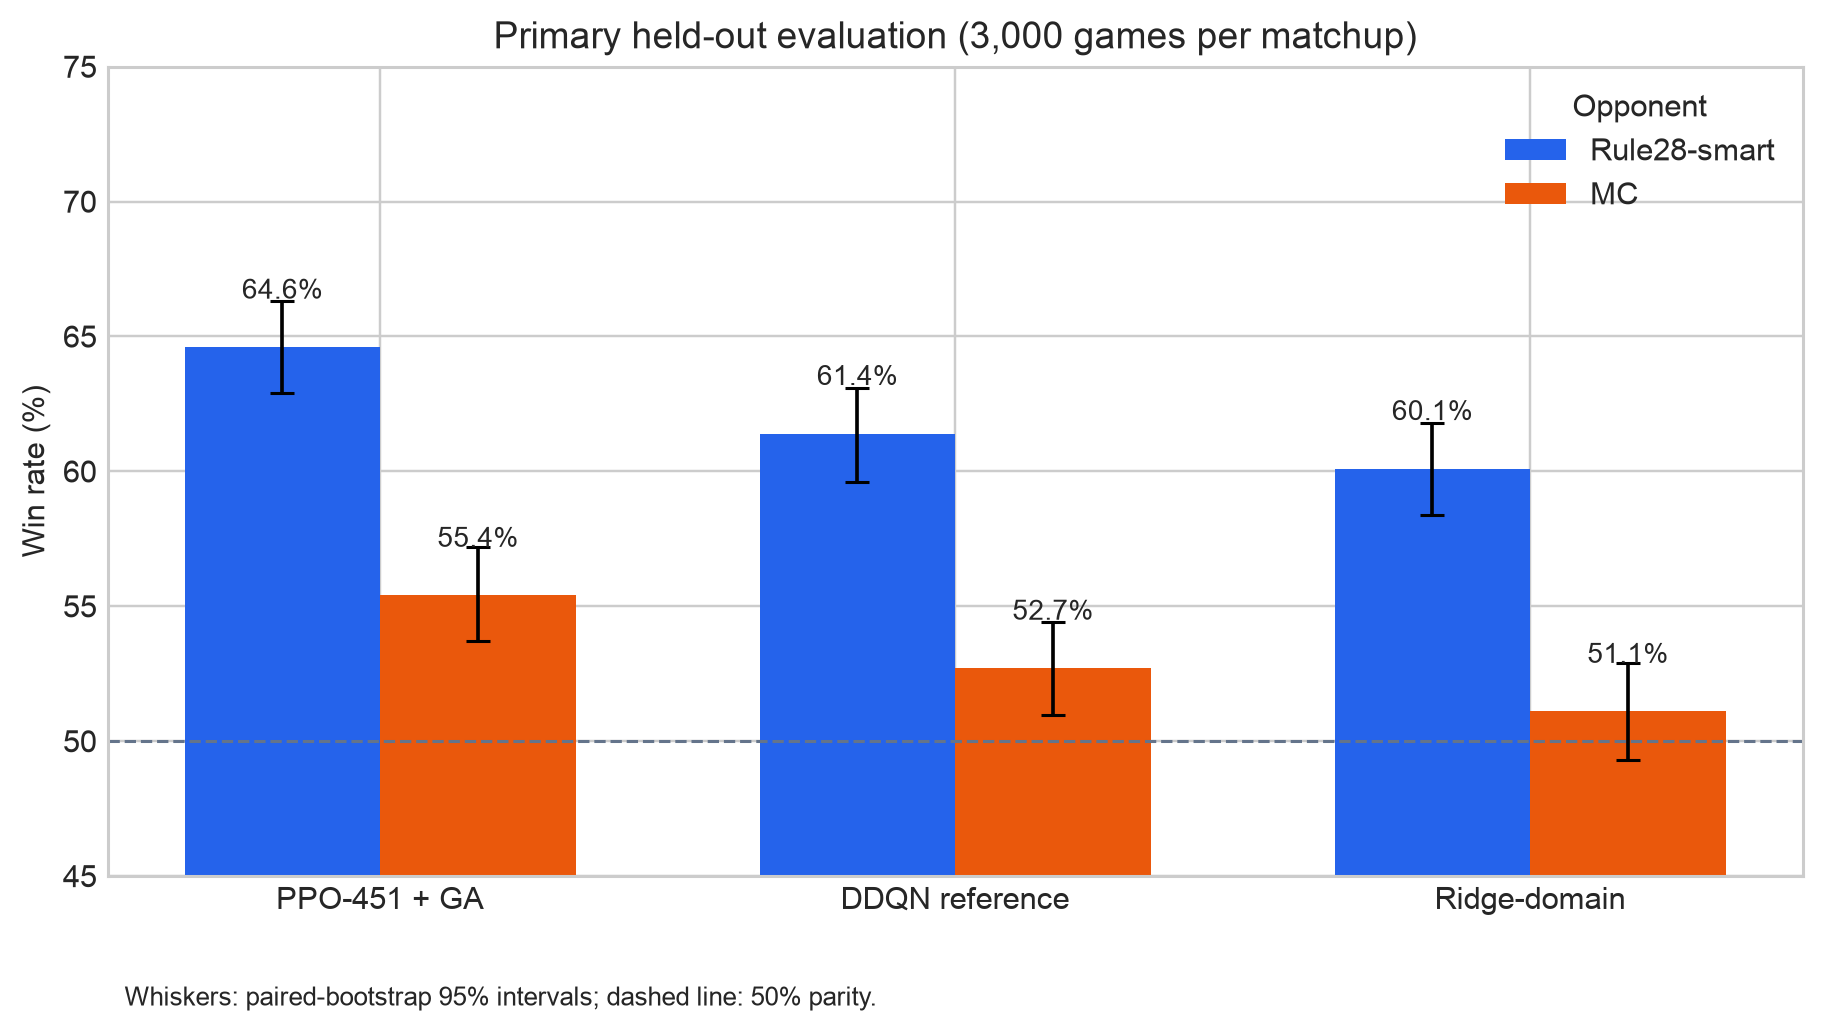
\includegraphics[keepaspectratio,alt={Primary held-out win rates with paired-bootstrap intervals.}]{figures/primary_evaluation.png}}

\textbf{Figure 1.} PPO has the highest point estimate against both
primary opponents, and its paired intervals are above the DDQN and Ridge
comparisons reported below.

PPO\textquotesingle s paired advantage over DDQN was \textbf{+3.2
points} against Rule28-smart, with a 95\% interval of \textbf{+1.2 to
+5.3}, and \textbf{+2.7 points} against MC, with an interval of
\textbf{+0.6 to +5.0}. PPO\textquotesingle s advantage over Ridge was
+4.5 points against Rule28-smart (interval +2.2 to +6.7) and +4.3 points
against MC (interval +1.9 to +6.6). DDQN versus Ridge was not
statistically resolved.

The primary PPO results were not merely wins against weak opponents. In
a separate 3,000-game external-opponent evaluation, PPO won 80.9\%
against the released Glenn--Aloi agent and 65.8\% against the
Couto-GA-stop adaptation. The corresponding PPO rates against
Rule28-smart and MC were 64.1\% and 55.3\%. These results also show
opponent dependence: Ridge slightly exceeded PPO against Glenn--Aloi
(81.7\% versus 80.9\%) in that evaluation.

\subsubsection{4.3 Additional-seed
robustness}\label{43-additional-seed-robustness}

We retrained each retained family with two additional seeds and
evaluated on a common fresh set of 3,000 games per matchup (seed
\texttt{20261101}). The values below are means over the two new training
seeds, not pooled games and not a claim that every future seed will
match them.

{\def\LTcaptype{none} % do not increment counter
\begin{longtable}[]{@{}lrrrr@{}}
\toprule\noalign{}
Model family & Rule28-smart mean & MC mean & External-opponent mean &
Minimum mean \\
\midrule\noalign{}
\endhead
\bottomrule\noalign{}
\endlastfoot
PPO (seeds 460/461) & \textbf{64.25\%} & 55.35\% & 74.6\% & 55.35\% \\
DDQN (seeds 448/449) & 59.50\% & 50.40\% & 71.0\% & 50.40\% \\
Ridge (seeds 642/643) & 63.25\% & \textbf{55.55\%} & \textbf{74.9\%} &
\textbf{55.55\%} \\
\end{longtable}
}

\pandocbounded{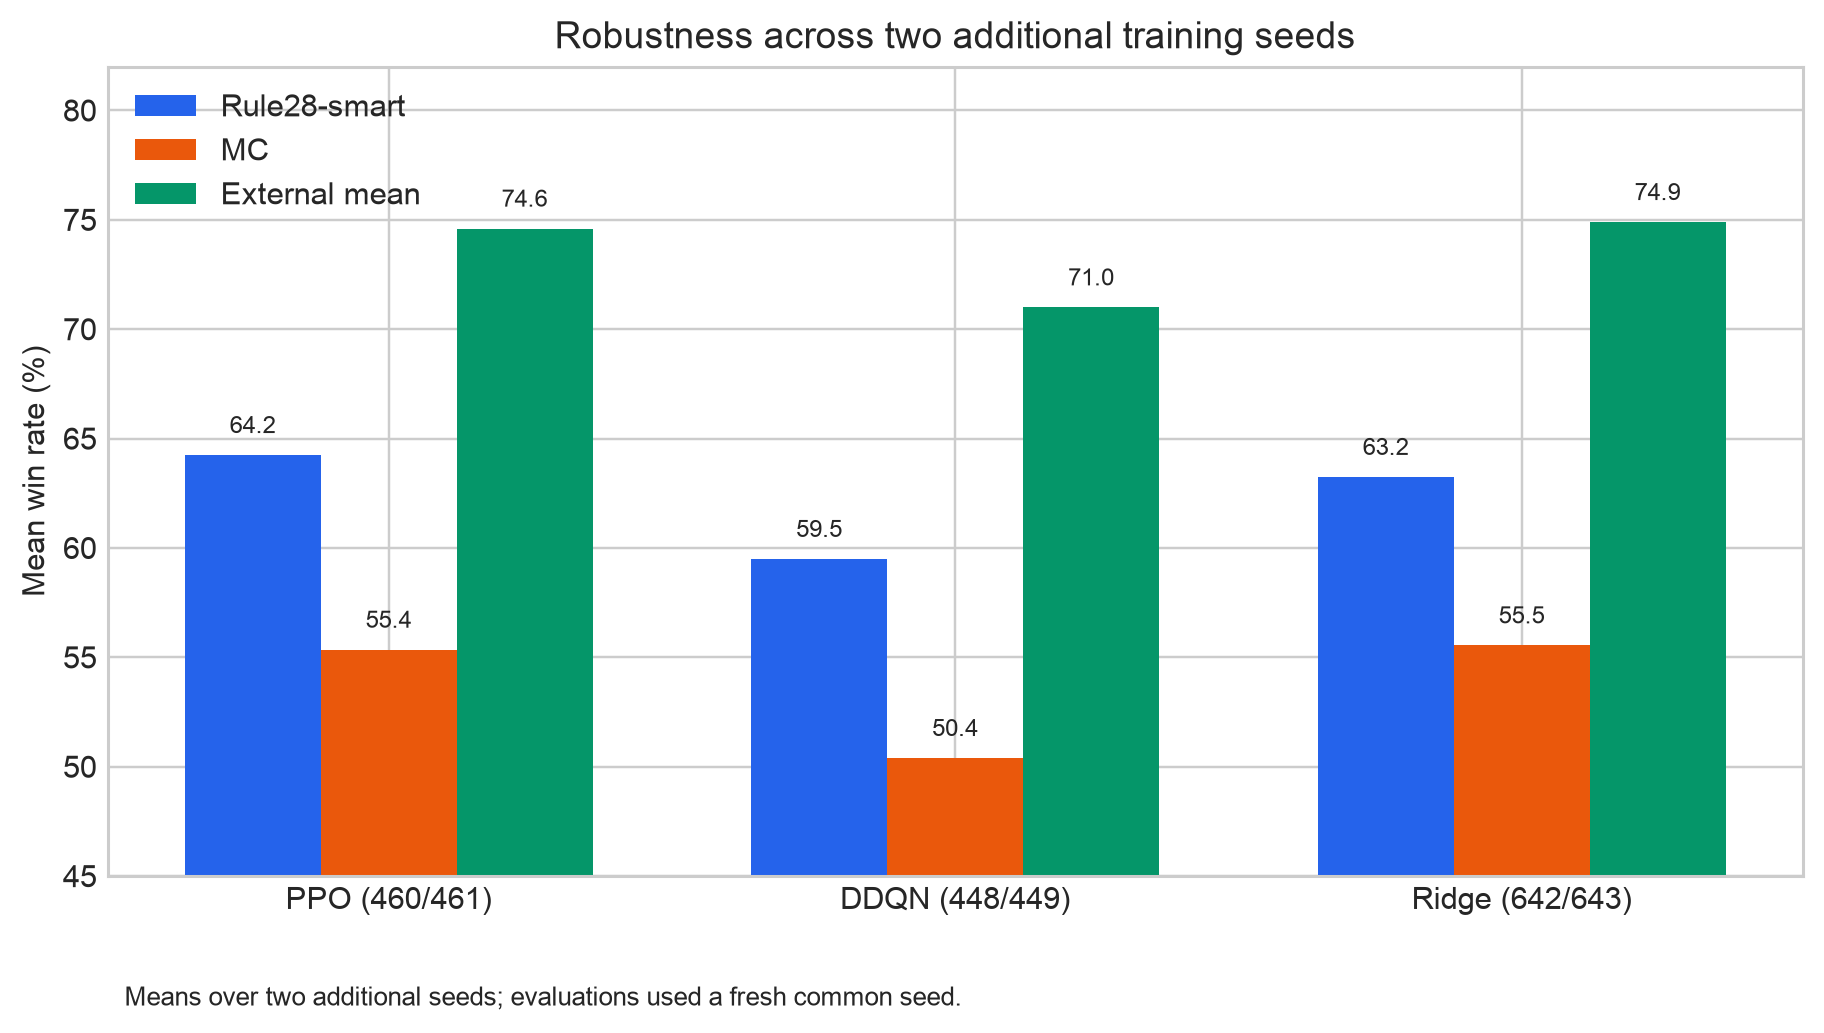
\includegraphics[keepaspectratio,alt={Mean win rates for two additional training seeds.}]{figures/seed_robustness.png}}

\textbf{Figure 2.} The additional-seed check shows that PPO and Ridge
are close, while DDQN has the lowest mean and greater seed sensitivity.

PPO was consistent across the two additional seeds. DDQN was more seed
sensitive, while Ridge was also stable and close to PPO. Thus the
evidence supports PPO as the strongest promoted RL policy, but not as a
uniformly dominant policy family.

\subsubsection{4.4 Direct head-to-head
results}\label{44-direct-head-to-head-results}

The six additional checkpoints were also compared directly in 3,000-game
pairings using seed \texttt{20261102}. Averaging the two cross-family
results gives:

{\def\LTcaptype{none} % do not increment counter
\begin{longtable}[]{@{}lr@{}}
\toprule\noalign{}
Pair & Approximate first-model win rate \\
\midrule\noalign{}
\endhead
\bottomrule\noalign{}
\endlastfoot
PPO versus DDQN & 56.1\% \\
PPO versus Ridge & 49.2\% \\
Ridge versus DDQN & 56.3\% \\
\end{longtable}
}

The direct results qualify the primary-opponent conclusion. Performance
is non-transitive and depends on the opponent; PPO is clearly strong
against the selected external baselines, but the new Ridge checkpoints
were competitive and slightly favored in direct games.

\pandocbounded{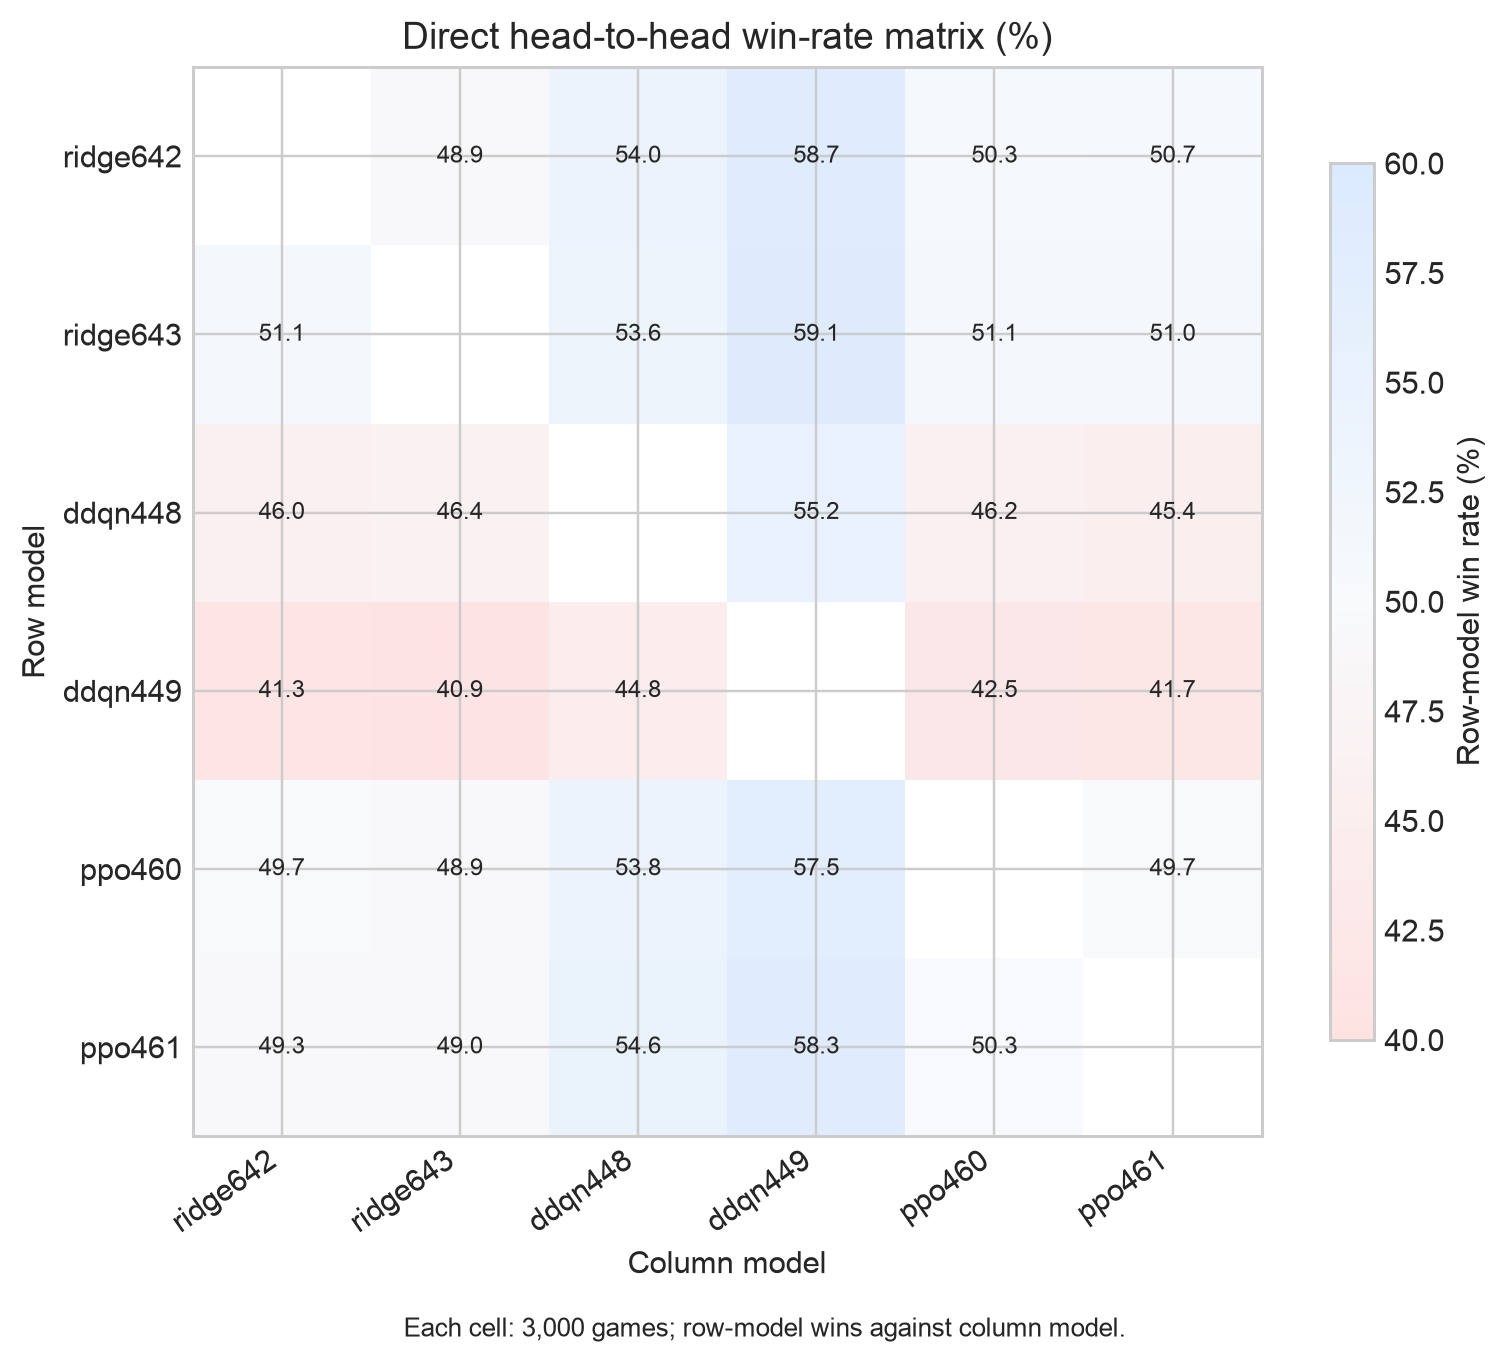
\includegraphics[keepaspectratio,alt={Direct head-to-head win-rate heatmap.}]{figures/head_to_head_heatmap.png}}

\textbf{Figure 3.} Rows are the models whose wins are counted; columns
are their opponents. The matrix makes the non-transitive relationship
visible instead of reducing it to one overall ranking.

\subsubsection{4.5 Ablations and negative
results}\label{45-ablations-and-negative-results}

Negative results were retained as part of the model-selection evidence:

\begin{itemize}
\tightlist
\item
  A learned-pairing PPO run destroyed performance when all parameters
  were updated. A pairing-only diagnostic preserved the Stop/Continue
  policy but still scored only 50.4\% versus Rule28-smart and 44.5\%
  versus MC, below PPO (64.6\% and 55.4\%) and DDQN (61.4\% and 52.8\%).
\item
  A supervised DNN trained on the original counterfactual dataset scored
  42.7\% and 36.2\% against Rule28-smart and MC, despite 68.2\%
  validation action accuracy. The multi-policy DNN was weaker still at
  32.3\% and 28.7\%.
\item
  Multi-policy Ridge improved over the original Ridge (62.7\%/57.4\%
  versus 59.4\%/53.2\% in its comparison), showing that
  state-distribution curation helped the linear model but did not make
  the DNN effective.
\item
  Self-play, conservative fine-tuning, targeted fine-tuning,
  reference-replay fine-tuning, and a counterfactual PPO screen all
  regressed on held-out games. For example, the reference-replay DDQN
  fell to 58.6\%/50.4\%/46.7\% against Rule28-smart/MC/Ridge.
\end{itemize}

These ablations prevent us from attributing all improvement to
neural-network capacity or to additional training alone.

\pandocbounded{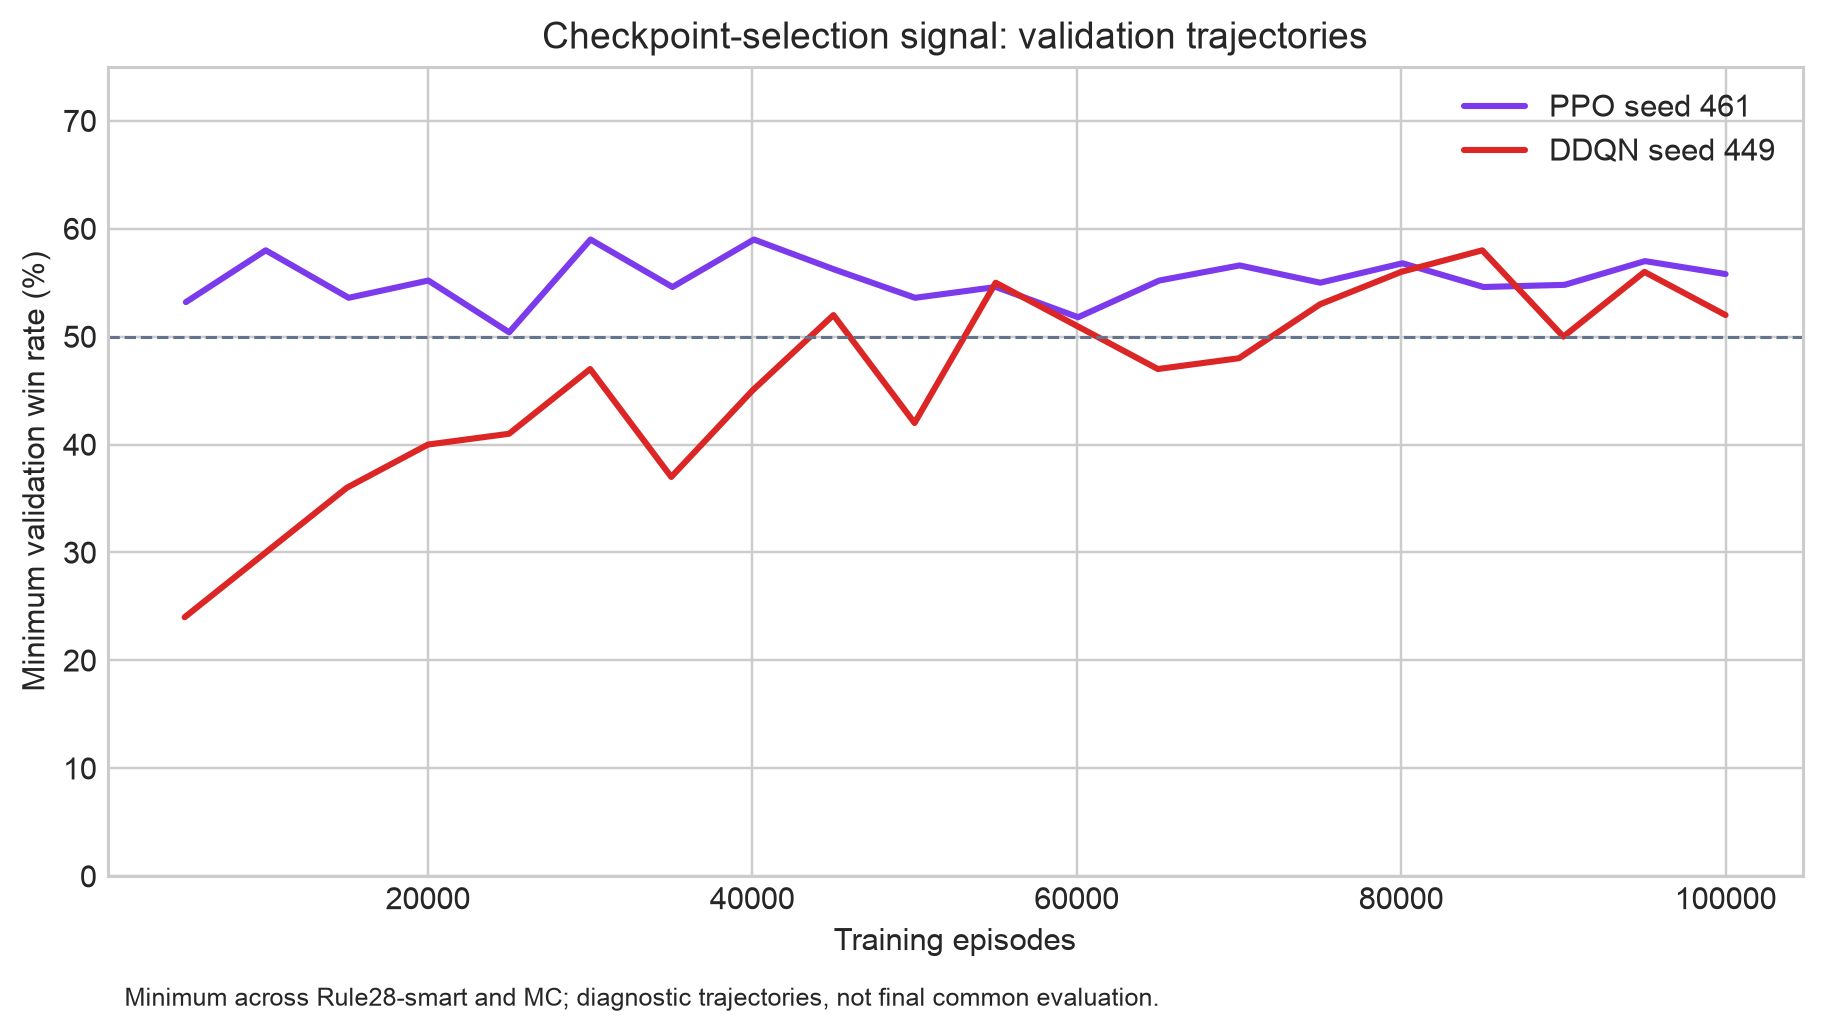
\includegraphics[keepaspectratio,alt={Minimum validation win-rate trajectories.}]{figures/validation_trajectories.png}}

\textbf{Figure 4.} Validation performance is noisy and
checkpoint-sensitive. This is why the final selection used a held-out
common evaluation rather than the last training checkpoint.

\subsection{5. Discussion}\label{5-discussion}

The answer to our research question is \textbf{qualified yes}. PPO
learned a stronger Stop/Continue policy than the retained DDQN and Ridge
baselines when tested against the primary heuristic and approximate MC
opponents. The advantage was statistically supported in the paired
common evaluation and was largely reproduced by two additional PPO
training seeds.

The answer is not ``PPO always wins.'' First, direct head-to-head
results are near 50--50 against Ridge and show non-transitive strategy
interactions. Second, the paired intervals are based on shared dice-seed
pairs and should not be interpreted as independent-game confidence
intervals. Third, training and evaluation use simulator-generated games,
so the conclusions concern this implementation of two-player
\emph{Can\textquotesingle t Stop}, fixed GA pairing, and the selected
opponent distribution.

The most useful engineering result is that selecting a stable checkpoint
and curating state distributions mattered more than adding model
complexity. Learned pairing was unsuccessful under the current
terminal-reward setup, while multi-policy data improved Ridge. The final
application should therefore ship PPO-451 + GA as the primary player,
keep DDQN as an RL reference, and offer Ridge as a lightweight
alternative.

\subsection{6. Limitations and Future
Work}\label{6-limitations-and-future-work}

\begin{enumerate}
\def\labelenumi{\arabic{enumi}.}
\tightlist
\item
  The main study uses two players and fixed GA dice pairing; a learned
  joint pairing policy was tested but not solved.
\item
  MC is an approximate one-turn rollout agent, not full-game MCTS or an
  optimal oracle.
\item
  The supervised labels are approximate Rule28-smart rollouts, so
  offline accuracy is not a substitute for complete-game evaluation.
\item
  PPO and Ridge have only two additional retraining seeds in the final
  robustness check. More independent seeds would strengthen
  generalization claims.
\item
  The current proof of concept has no graphical interface and does not
  claim support for three- or four-player variants.
\end{enumerate}

Future work should investigate legal-action-masked pairing with a better
training objective, broader independent-seed evaluation, and calibrated
explanations of the predicted risk of continuing.

\subsection{7. Reproducibility}\label{7-reproducibility}

The source tree contains the simulator, agents, training scripts, tests,
model checkpoints, raw per-game CSV files, JSON summaries, and
configuration files. The most important artifacts are:

\begin{itemize}
\tightlist
\item
  \texttt{cant\_stop\_baselines/docs/EXPERIMENT\_STATUS.md} ---
  experiment log and final decisions;
\item
  \texttt{cant\_stop\_baselines/runs/final\_common\_eval\_seed1000454/}
  --- primary common evaluation and raw games;
\item
  \texttt{cant\_stop\_baselines/runs/final\_retrain\_head\_to\_head\_seed20261102/}
  --- additional-seed direct comparisons;
\item
  \texttt{cant\_stop\_baselines/runs/ppo\_mc\_focused\_seed451/top\_1.pt}
  --- promoted PPO;
\item
  \texttt{cant\_stop\_baselines/runs/ddqn\_mc\_counterfactual\_seed447/best.pt}
  --- DDQN reference;
\item
  \texttt{cant\_stop\_baselines/runs/ridge\_multi\_policy\_seed642/} and
  \texttt{seed643/} --- additional Ridge models.
\end{itemize}

From \texttt{cant\_stop\_baselines/}, the regression suite can be run
with:

\begin{Shaded}
\begin{Highlighting}[]
\ExtensionTok{python3} \AttributeTok{{-}m}\NormalTok{ unittest discover }\AttributeTok{{-}s}\NormalTok{ tests }\AttributeTok{{-}t}\NormalTok{ . }\AttributeTok{{-}v}
\end{Highlighting}
\end{Shaded}

\subsection{8. Acknowledgements and
Contributions}\label{8-acknowledgements-and-contributions}

We acknowledge the authors of the Rule of 28, Glenn--Aloi heuristic, and
Couto/Sketch-SA(O) work cited below. Their methods are used as
documented baselines or adaptations; they are not presented as our
original algorithms.

\textbf{Contributions:} \emph{{[}replace this paragraph with each
member\textquotesingle s concrete work, for example simulator/rules,
data pipeline, PPO/DDQN training, evaluation, analysis, and report/video
preparation.{]}}

\subsection{References}\label{references}

\begin{enumerate}
\def\labelenumi{\arabic{enumi}.}
\tightlist
\item
  Martin Keller. ``Can\textquotesingle t Stop? Try The Rule of 28.''
  1986.
\item
  James Glenn and Christian Aloi. ``A Generalized Heuristic for
  Can\textquotesingle t Stop.'' FLAIRS, 2009.
  \url{https://cdn.aaai.org/ocs/123/123-2430-1-PB.pdf}
\item
  Leandro C. Medeiros, David S. Aleixo, and Levi H. S. Levis. ``What Can
  We Learn Even From the Weakest? Learning Sketches for Programmatic
  Strategies.'' AAAI, 2022.
  \url{https://doi.org/10.1609/aaai.v36i7.20744}
\item
  J. Cameron Carter. ``Using Machine Learning to Optimize the Board Game
  Can\textquotesingle t Stop.'' 2026, user-provided thesis.
\end{enumerate}

\end{document}
